\documentclass{article}


\usepackage{arxiv}

\usepackage[utf8]{inputenc} % LaTeX source encoded as UTF-8
\usepackage[czech]{babel}
\usepackage[T1]{fontenc}    % use 8-bit T1 fonts
\usepackage{hyperref}       % hyperlinks
\usepackage{url}            % simple URL typesetting
\usepackage{booktabs}       % professional-quality tables
\usepackage{amsfonts}       % blackboard math symbols
\usepackage{nicefrac}       % compact symbols for 1/2, etc.
\usepackage{microtype}      % microtypography
\usepackage{lipsum}
\usepackage[pdftex]{graphicx} 

\title{Reinforced learning}

\widowpenalty10000
\clubpenalty10000
\author{
  Ladislav Martínek\\
  \texttt{martilad@fit.cvut.cz} \\
  \\
  
\includegraphics[width=.16\textwidth]{./img/cvut-logo-bw}
  \\
  České vysoké učení technické v Praze\\
  Fakulta informačních technologií\\
  Katedra aplikované matematiky\\  
  %% examples of more authors
  %% \AND
  %% Coauthor \\
  %% Affiliation \\
  %% Address \\
  %% \texttt{email} \\
}

\begin{document}
\maketitle

\begin{abstract}
todo: write abstract
\end{abstract}


% keywords can be removed
\keywords{reinforcment learning \and zpětnovazební učení \and machine learning \and strojové učení \and posilové učení \and umělá inteligence}


\section{Úvod}
Když se zkusíme zamysled nad tím jak jsme se odmalička učili a jak učení probíhalo, tak nás jako první metoda napadne právě Reinforcment learning (dále budu používat zkratku RL), neboli také učení na základě zpětné vazby. Určitě jsme učení takto přímo nenazývali, ale zpětnou vazbu dostáváme odmalička. Zpětnou vazbou může být například když cítíme chlad pokud se dotkneme sněhu, které máme přímo od prostředí. Další zpětnou vazbu můžeme dostavat například od rodičů a určitou zpětnou vazbu od prostředí dostaváme téměř neustále. Na tomto způsobu je založena jedno z hlavních paradigmat strojového učení. V tomto případě nejsou systému poskytnutnuto žádné mapovaní správných odpovědí na daný vstup nebo interakci. Učený subjekt musí vyzkoušet, co mu přinese nějvětší užitek. V této práci popíši RL ve strojovém učení i s problémy, se kterými potýká, a podobnosti a odlišnosti s tímto učením u lidí. 


\section{Reinforcment learning}
\label{sec:headings}

Reinforcment learning v češtině také zpětnovazebné učení nebo posilové učení je způsob učení na základě odezvy a zpětné vazby z prostředí, ve které se učený subjekt pohybuje. 

Teorie RL poskytuje normativní pohled, který je hluboce zakořeněn v psychologickém a neurovědním pohledu na chování zvířat, jak mohou optimalizovat svoje chování a kontrolovat prostředí \cite{mnih2015human}. 

V rámci strojového učení se jedná přímo o jedno z paradigmat učení, které je v poslední době vělice popularní současně s tím jak roste výkon počítačů a je možné simulovat agenty a prostředí mnohem lépe. Na stejné úrovni rozdělení jako RL stojí učení s učitelem (angl. supervised learning) a učení bez učitele (angl. unsupervised learning). Oproti učení s učitelem (jeden z nejčastějších přístupů ve strojovém učení) není v RL poskytnut popis jednotlivých situací, ke kterým je určena ta správná akce. Rozdíl oproti učení bez učitelel je ten, že učení bez učitele slouží většinou k nalezení struktury v neoznačených datech \cite{sutton1998introduction}.

V RL zpětnou vazbu nejčastěji představují odměny nebo tresty. Učení je možné buď s obojím nebo například jen s odměnami nebo tresty. Učený subjekt se snaží o maximalizaci takové odměny nebo minimalizaci trestů. 

Podle \cite{sutton1998introduction} učený agent musí být schopen vnímat stav svého prostředí a musí být schopen provádět akce, které toto prostředí mění. Celkově je také agent řízen svými cíly, kterých se snaží dosáhnout a může k tomu využít různých cest, které můžou vytvořit různé cesty pro různé agenty.

Ze všech forem ML, RL je nejblíže tomu, ja se reálně učí lidé a ostatní zvířata. Mnoho postupů a myšlenka RL byla původně inspirována právě biologický systémem učení \cite{sutton1998introduction}. I ostatní části ML lze nalézt v biologickém systému, ale ty jsou především tom našel lidském, kde můžeme mít například učení s učitelem, kde se učime z příkladů, kde známe správné výsledky. Toto jsou pouze malé části, protože za nějakou takto naučenou látku jsme ve škole byly odměněni známkou nebo body. Dostali jsme zpětnou vazbu jestli zpusob jakým jsme se učili nebo kolik jsme tomu věnovali byl dostatečný a správný, či nikoliv.

 
\section{Reprezentace a simulace RL}

Když se podíváme na RL v našem životě, tak lze hodně jednoduše zobrazit pomocí obrázku \ref{zavislostKnnRec}. Většinu částí jsem již zmínil v \ref{sec:headings}. Ale v této části popíši jednotlivé součásti RL a jejich rozdíly mezi reálným světem a jejich simulací v počítači. Bude se jednat o agenta a prostředí, v rámci kterých popíši interpretace stavu prostředí a odměny pro agenta.
Dále agent musí mít nějaké cíle, kterých se snaží dosáhnout. Tyto cíle musí být staženy vždy na daný stav prostředí, ve kterém se nachází. Ty jsou nutné proto, aby agent měl nějaký směr (volbu akcí), kterým se vydat. 

\subsection{Prostředí}

\begin{figure}\centering
	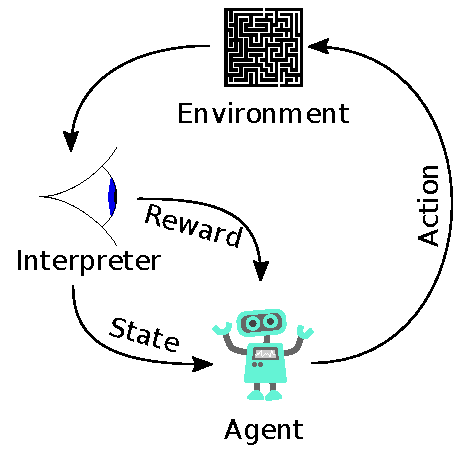
\includegraphics[width=0.25\textwidth]{img/RLdiagram}
 	\caption[]{Clasický scénář RL. Agent prování akce v prostředí, které je nějakým způsobem interpretováno. Z interpretace je odvozena odměna pro agenta a reprezentace stavu prostředí, který má agent k dispozici. \cite{pict} }\label{zavislostKnnRec}
 \end{figure}	


Ve strojovém učení (dále jen ML) je v \cite{sutton1999reinforcement} jako první zmíněna funkce generující odměnu pro agenta (nutná součást prostředí), protože každý agent je na základě svých akcích odměnován. V ML je nejčastěji odměnou celé číslo, které se spjato s nějakým stavem a akcí. Stavem je popsáno aktuální prostředí, které muže daný agent pozorovat např. rozehraná šachová partie. Ja je vidět na obrázku \ref{zavislostKnnRec}, stav je nějak interpretován a to nejčastěji nějakými senzory agenta.
 

Odměna pro agenta je vždy svázána se stavem a konkrétní akcí. Tento koncept stavů a akcí je velice obecný. Akce je  agentovo jakékoliv rozhodnutí, které agent může vykonat s stav je jakýkoliv fakt, který může vzít agent v úvahu při rozhodování \cite{sutton1999reinforcement}. 

V ML je ohodnocení poměrně omezené oproti reálnému světu. Zpětnou vazbu můžeme rozdělit například na Objektivní a subjektivní zpětnou vazbu. Při objektivní zpětné vazbě nevznikají pochyby a v případě ML je zpětná vazba vdy objektivní daná funkcí. Například tabulka s jasně danými odměnami. Subjektivní zpětná vazba může vyvolat pochyby o její důležitosti a pravosti, muže to být napřiklad pouze špatné rozhodnutí. V biologickém světě je mnohem častější. Jako příklad mě napadájí například odměny v práci, které můžou představovat objektivní zpětnou vazbu, kdy je závislá na počtu vyrobených kusů. Nebo subjektivní, kdy rozhoduje napřiklad manažer nad vámi.

Například při výcviku psa by jako pozitivní vazba pochvala příliž nefungovala, ale na nějaký pamlsek už reaguje většina psů. U lidí je množina možných odměn ještě rozsáhlejší a může být představována slovní pochvalou, finanční odměnou a mnoho dalšími. Vytvořit funkci v ML, která by toto zahrnovala je velice optížné až nemožné. Prostředí s odměnami je omezováno a většinou vždy specializováno na pár konkrétních cílů, kterých se daří dosahovat po učení. Více v kapitole \ref{sec:priklady}.


\subsection{Agent}
Agent je součástí konkrétního prostředí. Hlavním cílem agenta je mapování možných stavů na možné akce \cite{sutton1999reinforcement}. V ML může být implementováno například tabulkou nebo měnícím se prostředím. Jedná se asociace, které známe i z našeho života. 

Agenti mají většinou nějaké senzory, kterými pozorují okolní prostředí. Jako agenta v prostředí, můžeme například uvažovat samořídící auto, které má různé senzory, pomocí kterých se orientuje v prostoru (lidar, radar, kamery , atd\dots). Pro takového agenta je možné použít RL na jeho učení. Většinou není použito pouse RL, ale i další metody učení, tak že prostor akcí je striktně velmi omezen, protože provoz se zvázán zákony. Vazbu prostředí získavájí i zvířata a lidé. K získání stavu prostředí nám slouží oči, hmat, sluch, ale například i čich a další\dots 

Informace ze senzorů můžeme nazvat vnitřními nebo také vlastními. Na druhé straně jsou vnější, které můžeme získat od ostatních agentů jako ucelenou informaci. I s příkladem jsou více popsány v \ref{monkey}.


\section{Exploitation vs. Exploration}
Jak se píše v \cite{kaelbling1996reinforcement}, jeden z hlavních rozdílů mezi učením s učitelem a RL je, že v případě RL musí agent explicitně prozkoumávat prostředí akcemi. Potom je zasádní jaký udělá kompromis. Zdali bude prostředí velmi aktivně prozkoumávat (exprorace), ale za cenu mnohých neúspěchů nebo v případě, že nalezne akce, ze kterých plyne nějaký profit a začne se zaměřovat na tyto akce a provádět tzv. exploitaci. Může existovat mnoho různých akcí, které by mohli být optimálnější, ale pokud bude prozkoumávat pouze okolí těchto, tak na ně nikdy neodsáhne. Uvízne v tzv. lokálním maximu.

Když se podíváme do reálného světa můžeme vidět, že i tyto dva přístupy jsou zde vidět. Je to pozorovatelné jak mezi zvířaty tak mezi lidmi. Existují takový jedinci, kteří zkoušejí vše, co se jim nabídne nebo se snaží co nejvíce prozkoumat možnosti a hranice. K přirovnání k vedoucím manažerským pozicím to může být například způsob vedení firmy. Vysoká explorace může zapříčinit vysoký zisk, ale také je stejná možnost rychlého pádu při radikálních změnách směřování firmy a hledání optimální cesty. Na druhou stranu exploitace může pomoci upevnit pozici na konkrétním segmentu a stavu, ale růst firmy například již nebude tak rychlý, jakýho my se mohlo třeba dosáhnout vysokou explorací.

Agenti v ML musí volit nejen takové akce, které optimalizují zisk, ale také akce, které dovolí dostatečné prozkoumání prostoru. Každá akce musí být několikrát vyzkoušena, aby se zíkal statictický odhad její očekávané odměny \cite{sutton1998introduction}. V ML jsou metody využity především k řešení úloh, kde je žádoucí dosáhnout co nejlepšího výsledku, narozdíl od reálného světa, kde nemusí být ve výsledku takový problém uváznutí v lokálním maximu. Protože z pozice osoby (agenty) můžou být také akce optimální. Osoba je například spokojená, záleží pouze na cíli, který osoba má a může mít mnoho podob. Pro potřeby ML, kde je cíl a učel známý nám tedy explorace může pomoc se z takového lokálnímo maxima dostat. 


\section{Metody RL}
V této kapitole a především jejích podkapitolách popíši některé metody, které jsou v rámci RL používané. Tyto metody lze podle knihy \cite{sutton1998introduction} rozdělit na metody, kde jsou akcí a stavů není tolik a je možné je reprezentovat tabulkou. Tyto metody sjou schopny většinou nalézt přesné řešení v dáne množině akcí a stavů. Na druhé  raně jsou aproximační metody, které většinou najdou pouze přibližné řešení, ale za to je možné je použít na mnohem větší problémy. 


\subsection{Dynamické programování}
Dynamické programování je první z method pro řešení RL. Problém je formulován jako Markovův rozhodovací proces, na kterém je možné dynamické programování použít. Markovův proces je proces, který se skladá z mnnožiny stavů, akcí, pravděpodobnosti, že ve stavu $s$ bude provedena akce $a$ a okamžitý užitek po přechodu do nového stavu pro provedení konkrétní akce na současném stavu \cite{sutton1998introduction}. 

Dynamické programování je popsané v \cite{sutton1998introduction} a předpokladáme pro něj konečnou množinu stavů a akcí. V opačném případě je mroblém reprezentace v konečné paměti. Dynamické programování je založeno na principu, že podstrategie optímální strategie je opět optimální. Toto není použitelné na jakoukoliv úlohu, ale pro ty, kde platí, lze využít dynamické programování. 

V dynamickém programování jsme schopni výsledek většího podproblémuvyjadřit pomocí menších problému, které sme už jednou vyřešili, není tedy nutné některé jednoduché kony řešit opakovaně. V tomto je přímo vidět učení z normalního světa. Příklad mě napadá třeba, když dáme dítěti šroubovák a nějaké šroubky a prostor. Zaa chvíli se naučí jak se šroubovákem pracovat a tuto podúlohu poté použije v jakém koliv věku, když si bude stavět sřínku, ale člověk se nebude opakovaně učit šroubovat. Přesně tohodle principu je využito i při dynamickém programování, kde se výhradně pracuje s tabulkou, která je na základě stavů daného prostředí a možných akcí vypňována, až je dosaženo požadováného cíle.

\subsection{Monte carlo metody}
Monte carlo metody jsou stochastické metody, které jsou hojně využívané tam, kde není možné prozkoumávat celý stavový prostor souvisle. Narozdíl od přechozích části, zde nepředpokládáme znalost všech stavů a akcí, celkovou znalost prostředí. Monte carlo metody vyžadují pouze zkušenost, nějaký vzorek sekvencí stavů, akcí a odměn z aktuální interakce s prostředím \cite{sutton1998introduction}. Učení ze zkušenosti je velice překvapujícíc protože nevyžaduje zznalost dyamiky prostředí a přesto může dosáhnout dobrého řešení. I zde potřebujeme znát model, ale potřebujeme ho pouze ke generování ukázkových přechodů a nikoliv k rozdělení pravděpodobnosti do tabulky všech možných přechodů jako tomu bylo u dynamického programování. 

Je přimovyužito průmerovaní odměn za danou akci v daném prostředí. Model se učí z oddměn, které dostává. V monte carlo metodách je používána určitá složka náhody, která slouží k výběru akcí a prozkoumání prostoru s tím, že je upravována podle zkušenosti jaké bylo dosaženo. Akce bez odměny mohou být například jedno zopakovány a vyzkoušeny ale průmerováním budou velmi rychle vyloučeny. Pokud učíme psa, tak ho taky zkušeností naučíme, že třeba nesmí vyhrabávat koš, kde za takovou akci přijde ještě trest, tak již takové chování nikdy nezopakuje stejně tak se bude chovat agent v případě učení pomocí monte carlo metod. Více je videt v kapitole \ref{sec:priklady}. 


\subsection{Temporal difference (TD) learning}
TD je kombinací metod monte carlo učení a dynamického programování. Stejně jako v monte carlo metodách se může učit přímo ze zkušeností, tak také aktualizují tabulku částečných naučených akcích jako v dnamickém programování \cite{sutton1998introduction}. Algoritmy se mohou i navzájem prolínat a využívá se vždy silných stránek daneho algoritmu. TD upravují a vybírají akce podle toho jaký bude mít výsledek do budoucnosti, podle přechozích zjištěních a ještě dříve než je konečný výsledek znám. Monte carlo metody naopak rozhodují až podle výsldku, kterého dosáhly.


\subsection{Aproximační metody RL}




\section{Příklady RL}
\label{sec:priklady}

\subsection{human-level control}
\cite{mnih2015human}
\subsection{Open ai}
\cite{openAI}
\cite{baker2019emergent}
\subsection{monkeys}
\label{monkey}
 \cite{monkeyExp}
 \cite{hamel1996competing}

The documentation for \verb+natbib+ may be found at
\begin{center}
  \url{http://mirrors.ctan.org/macros/latex/contrib/natbib/natnotes.pdf}
\end{center}


\subsection{Závěr}
RL je velice populární metoda ve strojovém učení, ovšem jako všechny ostatní metody není všehschopná a má vlastní omezení a limity. První je především nutnost specifikovat množinu akcí, kterou jsou schopni agenti vykonávat a která je většinou neměnná. Dále je potřeba přesně specifikovat cíl. Může se stát, že problém bude tak komplexní, že bude problém cíl specifikovat.
todo: závěr taky bude 


\bibliographystyle{csn690}  
\bibliography{references}  
\end{document}